\documentclass[a4paper, 12pt]{article}
\usepackage[utf8]{inputenc}
\usepackage{amsmath,amsfonts,amsthm,amssymb,longtable,listings,graphicx, float, epstopdf, textcomp}
\usepackage{mathtools}
\usepackage[finnish]{babel}
\usepackage{tikz}
\renewcommand{\contentsname}{Sisällysluettelo}
\renewcommand{\abstractname}{Abstrakti}
\theoremstyle{definition}
\newtheorem{mydef}{Määritelmä}
\newtheorem{huom}{Huomautus}
\newtheorem{lemma}{Lemma}
\newtheorem{example}[mydef]{Esimerkki}
\theoremstyle{plain}
\newtheorem{teor}[mydef]{Lause}


\lstset{basicstyle=\small, frame=single}

\begin{document}

\title{Graafien automorfismiryhmä}
\author{Juuso Valli}
\date{24. 9. 2017}

\maketitle

\begin{abstract}
% TBW
\end{abstract}

\tableofcontents

\newpage

\section{Määritelmiä ja merkintöjä}

Olkoon $V$ äärellinen joukko. Olkoon $E(V) = \{\{u, v\} | u, v \in V, u \neq v\}$ joukon $V$ alijoukkojen joukko, jonka jäsenet sisältävät täsmälleen kaksi eri solmua.
Olkoon \emph{graafi} $G = (V, E), E \subseteq E(V)$. Joukkoa $V$ kutsutaan graafin $G$ \emph{solmuiksi}, ja joukkoa $E$ kutsutaan \emph{kaariksi}. Annetun graafin solmujoukosta kätetään merkintää $G_V$, ja kaarijoukosta merkintää $G_E$.
Kaaresta $\{u, v\}$ käytetään merkintää $uv$. Huomaa että näillä merkinnöillä $uv = vu$.
Yksinkertaisuuden vuoksi solmuista käytetään myös merkintää $v \in G$ merkinnän $v \in G_V$ sijaan.

Olkoon $G$ ja $H$ graafeja. Graafit $G$ ja $H$ ovat \emph{isomorfiset} $G \cong H$ mikäli on olemassa bijektio $f: V_G \rightarrow V_H$ siten, että
\begin{center}
\begin{math}
uv \in E_G \Longleftrightarrow f(u)f(v) \in E_H
\end{math}
\end{center}
kaikilla $u, v \in G$.

Tällaisia bijektioita kutsutaan \emph{isomorfismeiksi}.

Graafin $G$ \emph{automorfismit} ovat sen isomorfismeja itsensä kanssa. Triviaalisti nähdään että identiteettikuvaus on kaikkien graafien automorfismi, mutta graafeilla voi olla myös muita automorfismeja.

\begin{example}
\label{ex:d4}
Olkoon graafi $G = (\{v_1, v_2, v_3, v_4\}, \{v_1v_2, v_2v_3, v_3v_4, v_4v_1\})$.

\begin{center}
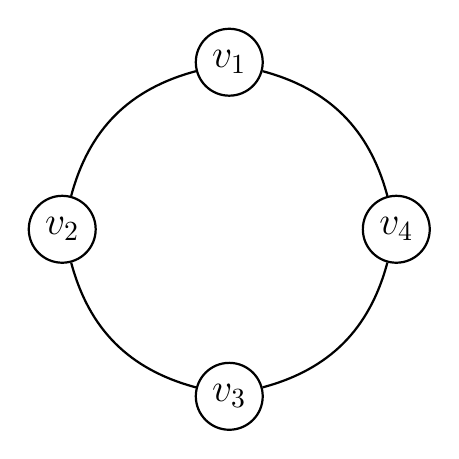
\begin{tikzpicture} [auto, node distance=3cm, every loop/.style={},
                    thick,solmu/.style={circle,draw,font=\sffamily\Large\bfseries}]

\node[solmu] (1) {$v_1$};
\node[solmu] (2) [below left of=1] {$v_2$};
\node[solmu] (3) [below right of=2] {$v_3$};
\node[solmu] (4) [below right of=1] {$v_4$};

 \path[every node/.style={font=\sffamily\small}]
    (1) edge [bend right] node[left] {} (2)
    (2) edge [bend right] node[left] {} (3)
    (3) edge [bend right] node[right] {} (4)
    (4) edge [bend right] node[right] {} (1);
\end{tikzpicture}
\end{center}

Olkoon kuvaus $f: V_G \rightarrow V_G, f(v_1) = v_2, f(v_2) = v_3, f(v_3) = v_4, f(v_4) = v_1$. Kuvaus $f$ on selvästi bijektio. Se, että kuvaus $f$ on automorfismi voidaan tarkistaa suoraan määritelmästä.

\begin{center}
\begin{tabular} {l l l}
$G_E$ & $f(u)f(v)$ & $f^{-1}(u)f^{-1}(v)$ \\
\hline
$v_1v_2$ & $ v_2v_3$ & $v_4v_1$ \\
$v_2v_3$ & $ v_3v_4$ & $v_1v_2$ \\
$v_3v_4$ & $v_4v_1$ & $v_2v_3$ \\
$v_4v_1$ & $v_1v_2$ &  $v_3v_4$ \\
\end{tabular}

\end{center}
\end{example}

\section{Automorfismiryhmä}

Olkoon $G_S$ graafin $G$ automorfismien joukko.

\begin{lemma}
\label{lemma:binaarirelaatio}
Kuvausten kompositio on binäärirelaatio $\circ : G_S \times G_S \rightarrow G_S$.
\begin{proof}
Olkoon $u, v \in G$. Olkoon $f, g \in G_S$.
\begin{center}
\begin{math}
uv \in E_G \xLeftrightarrow{g \in G_S} g(u)g(v) \in E_G  \xLeftrightarrow{f \in G_S} f(g(u))f(g(v)) \in E_G 
\end{math}
\end{center}
joten $f \circ g \in G_S$.
\end{proof}
\end{lemma}

\begin{lemma}
\label{lemma:identiteetti}
Jokaisella graafilla on identiteettikuvaus, joka on automorfismi.
\begin{proof}
Olkoon $u, v \in G$. Olkoon $id: G_V \rightarrow G_V, id(x) = x \forall x \in G_V$.
\begin{center}
\begin{math}
uv \in E_G \xLeftrightarrow{id(x) = x} id(u)id(v) \in E_G  
\end{math}
\end{center}
joten $id \in G_S$.
\end{proof}
\end{lemma}

\begin{lemma}
\label{lemma:kaanteiskuvaus}
Automorfismin $f$ käänteiskuvaus $f^{-1}$ on automorfismi.
\begin{proof}
Olkoon $u, v \in G$.
\begin{center}
\begin{math}
f^{-1}(u)f^{-1}(v) \in E_G \xLeftrightarrow{f \in G_S} f(f^{-1}(u))f(f^{-1}(v)) \in E_G \Leftrightarrow uv \in E_G
\end{math}
\end{center}
joten $f^{-1} \in G_S$.
\end{proof}
\end{lemma}

\begin{teor}
Pari $(G_S, \circ)$ on ryhmä.
\begin{proof}
Lemman \ref{lemma:binaarirelaatio} mukaan $\circ$ on $G_S$:n binäärirelaatio. Assosiatiivisuus on selvä kuvausten komposition assosiatiivisuuden perusteella. Lemman \ref{lemma:identiteetti} mukaan jokainen $G_S$ sisältää identiteettikuvauksen $id$, joka on ryhmän neutraalialkio. Lemman \ref{lemma:kaanteiskuvaus} mukaan jokaisella automorfismilla $f$ on käänteiskuvaus $f^{-1} \in G_S$.
\begin{center}
\begin{math}
\end{math}
\end{center}
\end{proof}
\end{teor}

Graafin automorfismiryhmää kutsutaan myös graafin symmetriaryhmäksi.

\begin{huom}
Graafien automorfismiryhmät eivät yleisesti ole kommutatiivisia.\\
Tämä nähdään helposti vastaesimerkin kautta. Tarkastellaan esimerkin \ref{ex:d4} mukaista graafia. Olkoon $f$ esimerkissä esitetty automorfismi. Olkoon kuvaus $g: V_G \rightarrow V_G, g(v_1) = v_1, g(v_2) = v_4, g(v_3) = v_3, g(v_4) = v_2$. Kuvaus $g$ on selvästi myös graafin $G$ automorfismi. Mikäli automorfismiryhmä olisi kommutatiiviinen, olisi $f \circ g = g \circ f$. Kirjoittamalla kuvaukset auki nähdään että $f \circ g(v_1) = f(g(v_1)) = f(v_1) = v_2$, mutta toisaalta $g \circ f (v_1) = g(f(v_1)) = g(v_2) = v_4$, mistä seuraa ristiriita.
\end{huom}

\begin{example}
Esimerkin \ref{ex:d4} mukaisen graafin symmetriaryhmä $G_S$ on isomorfinen diedriryhmän $D_4$ kanssa. Tämä nähdään helposti tarkastelemalla $G_S$:n ryhmätaulua. Otetaan $G_S$:n alkioille käyttöön seuraavat merkinnät: $\alpha_{n, i} \in G_S, 0 \geq n \lt4, i \in \{0, 1\} $, siten että $\alpha_{n, i}$

Yleisemmin $n$:n alkion rengasgraafien symmetriaryhmä on isomorfinen diedriryhmän $D_n$ kanssa.
\end{example}

\begin{example}
%TBW
Suoran graafin symmetriaryhmä on $C_2$
\end{example}

\begin{example}
%TBW
Puugraafin symmetriaryhmä on $C_2$
\end{example}

\section{Fruchtin teoreema}
%TBW

\end{document}